%%%%%%%%%%%%%%%%%%%%%%%%%%%%%%%%%%%%%%%%%%%%%%%%%%%%%%%%%%%%%%%%%%%%%%%%%%%%%%
%
% Section file included in main project file using \input{}
%
% Assumes that LaTeX2e macros and packages defined in cg_comp.sty are
%   available
%
%%%%%%%%%%%%%%%%%%%%%%%%%%%%%%%%%%%%%%%%%%%%%%%%%%%%%%%%%%%%%%%%%%%%%%%%%%%%%%

 \section{Experimental Estimate of the String Constant\label{sct:exp}}

 \begin{figure}
  \centering
  \begin{subfigure}[b]{0.45\textwidth}
      \centering
      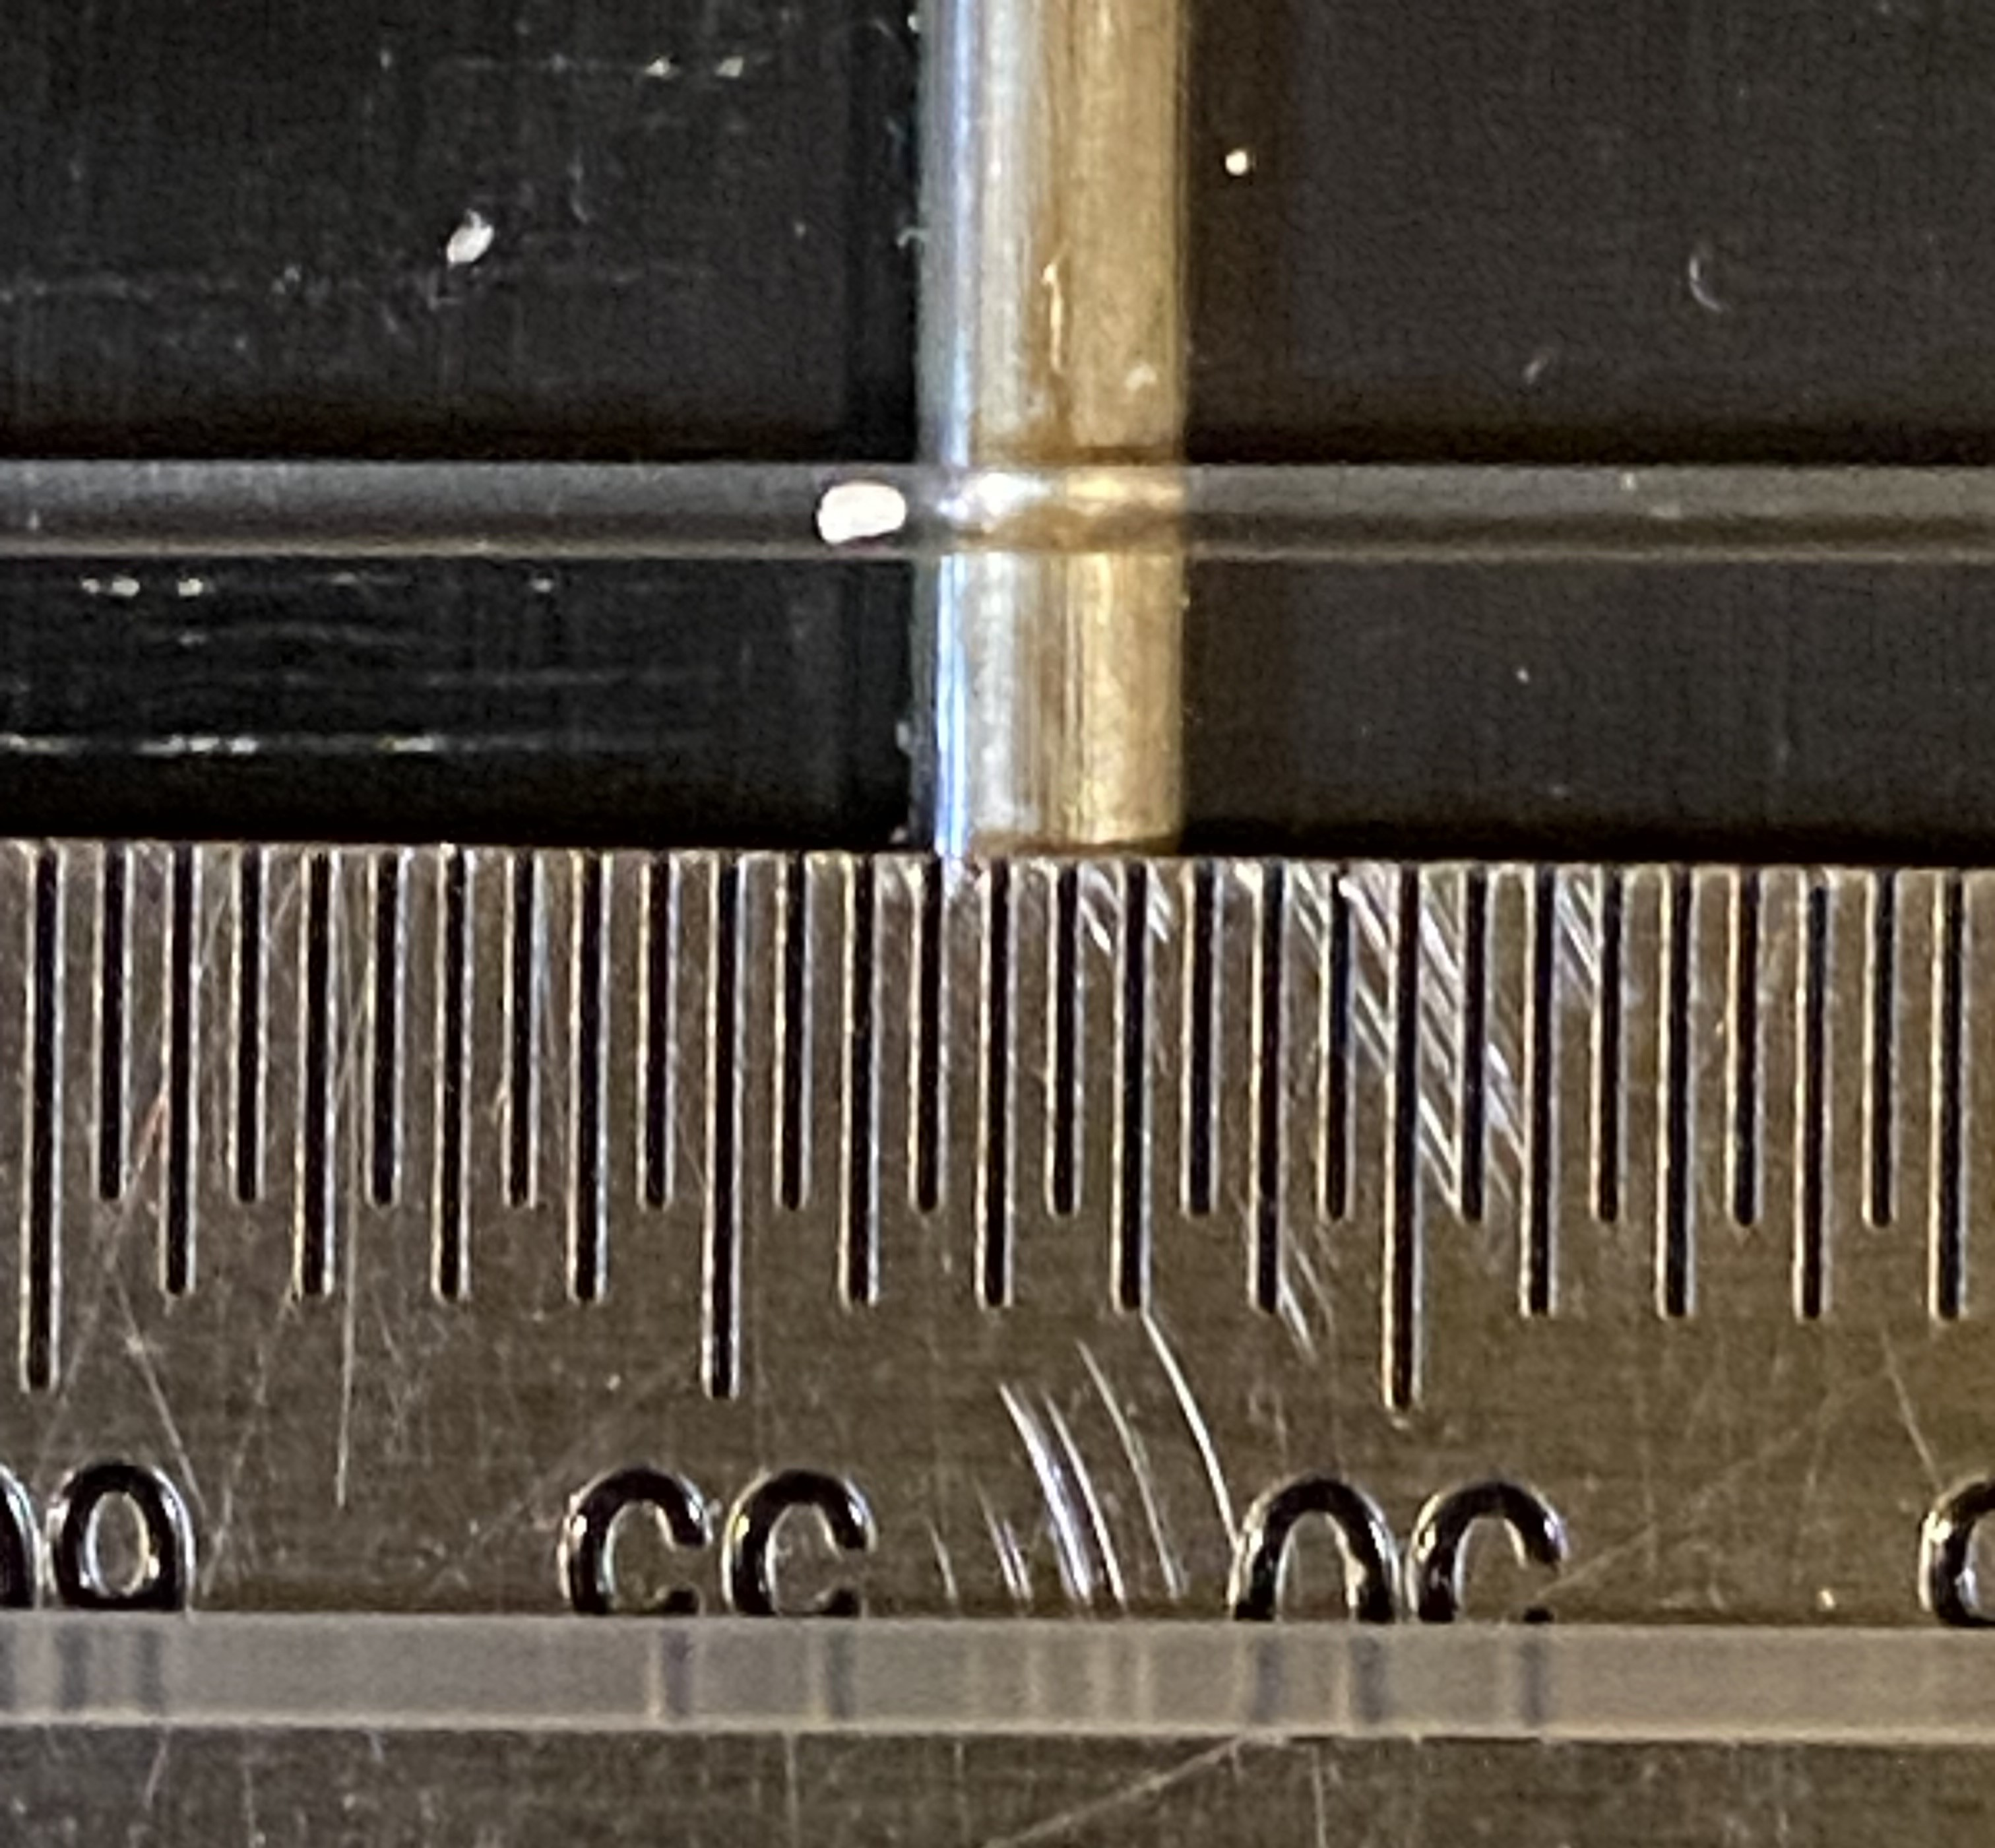
\includegraphics[width=3.0in]{figures/exp_dx1.jpg}
      \caption{$\Delta x_1$}
      \label{fig:exp_dx1}
  \end{subfigure}
  \hspace{0.25in}
  \begin{subfigure}[b]{0.45\textwidth}
      \centering
      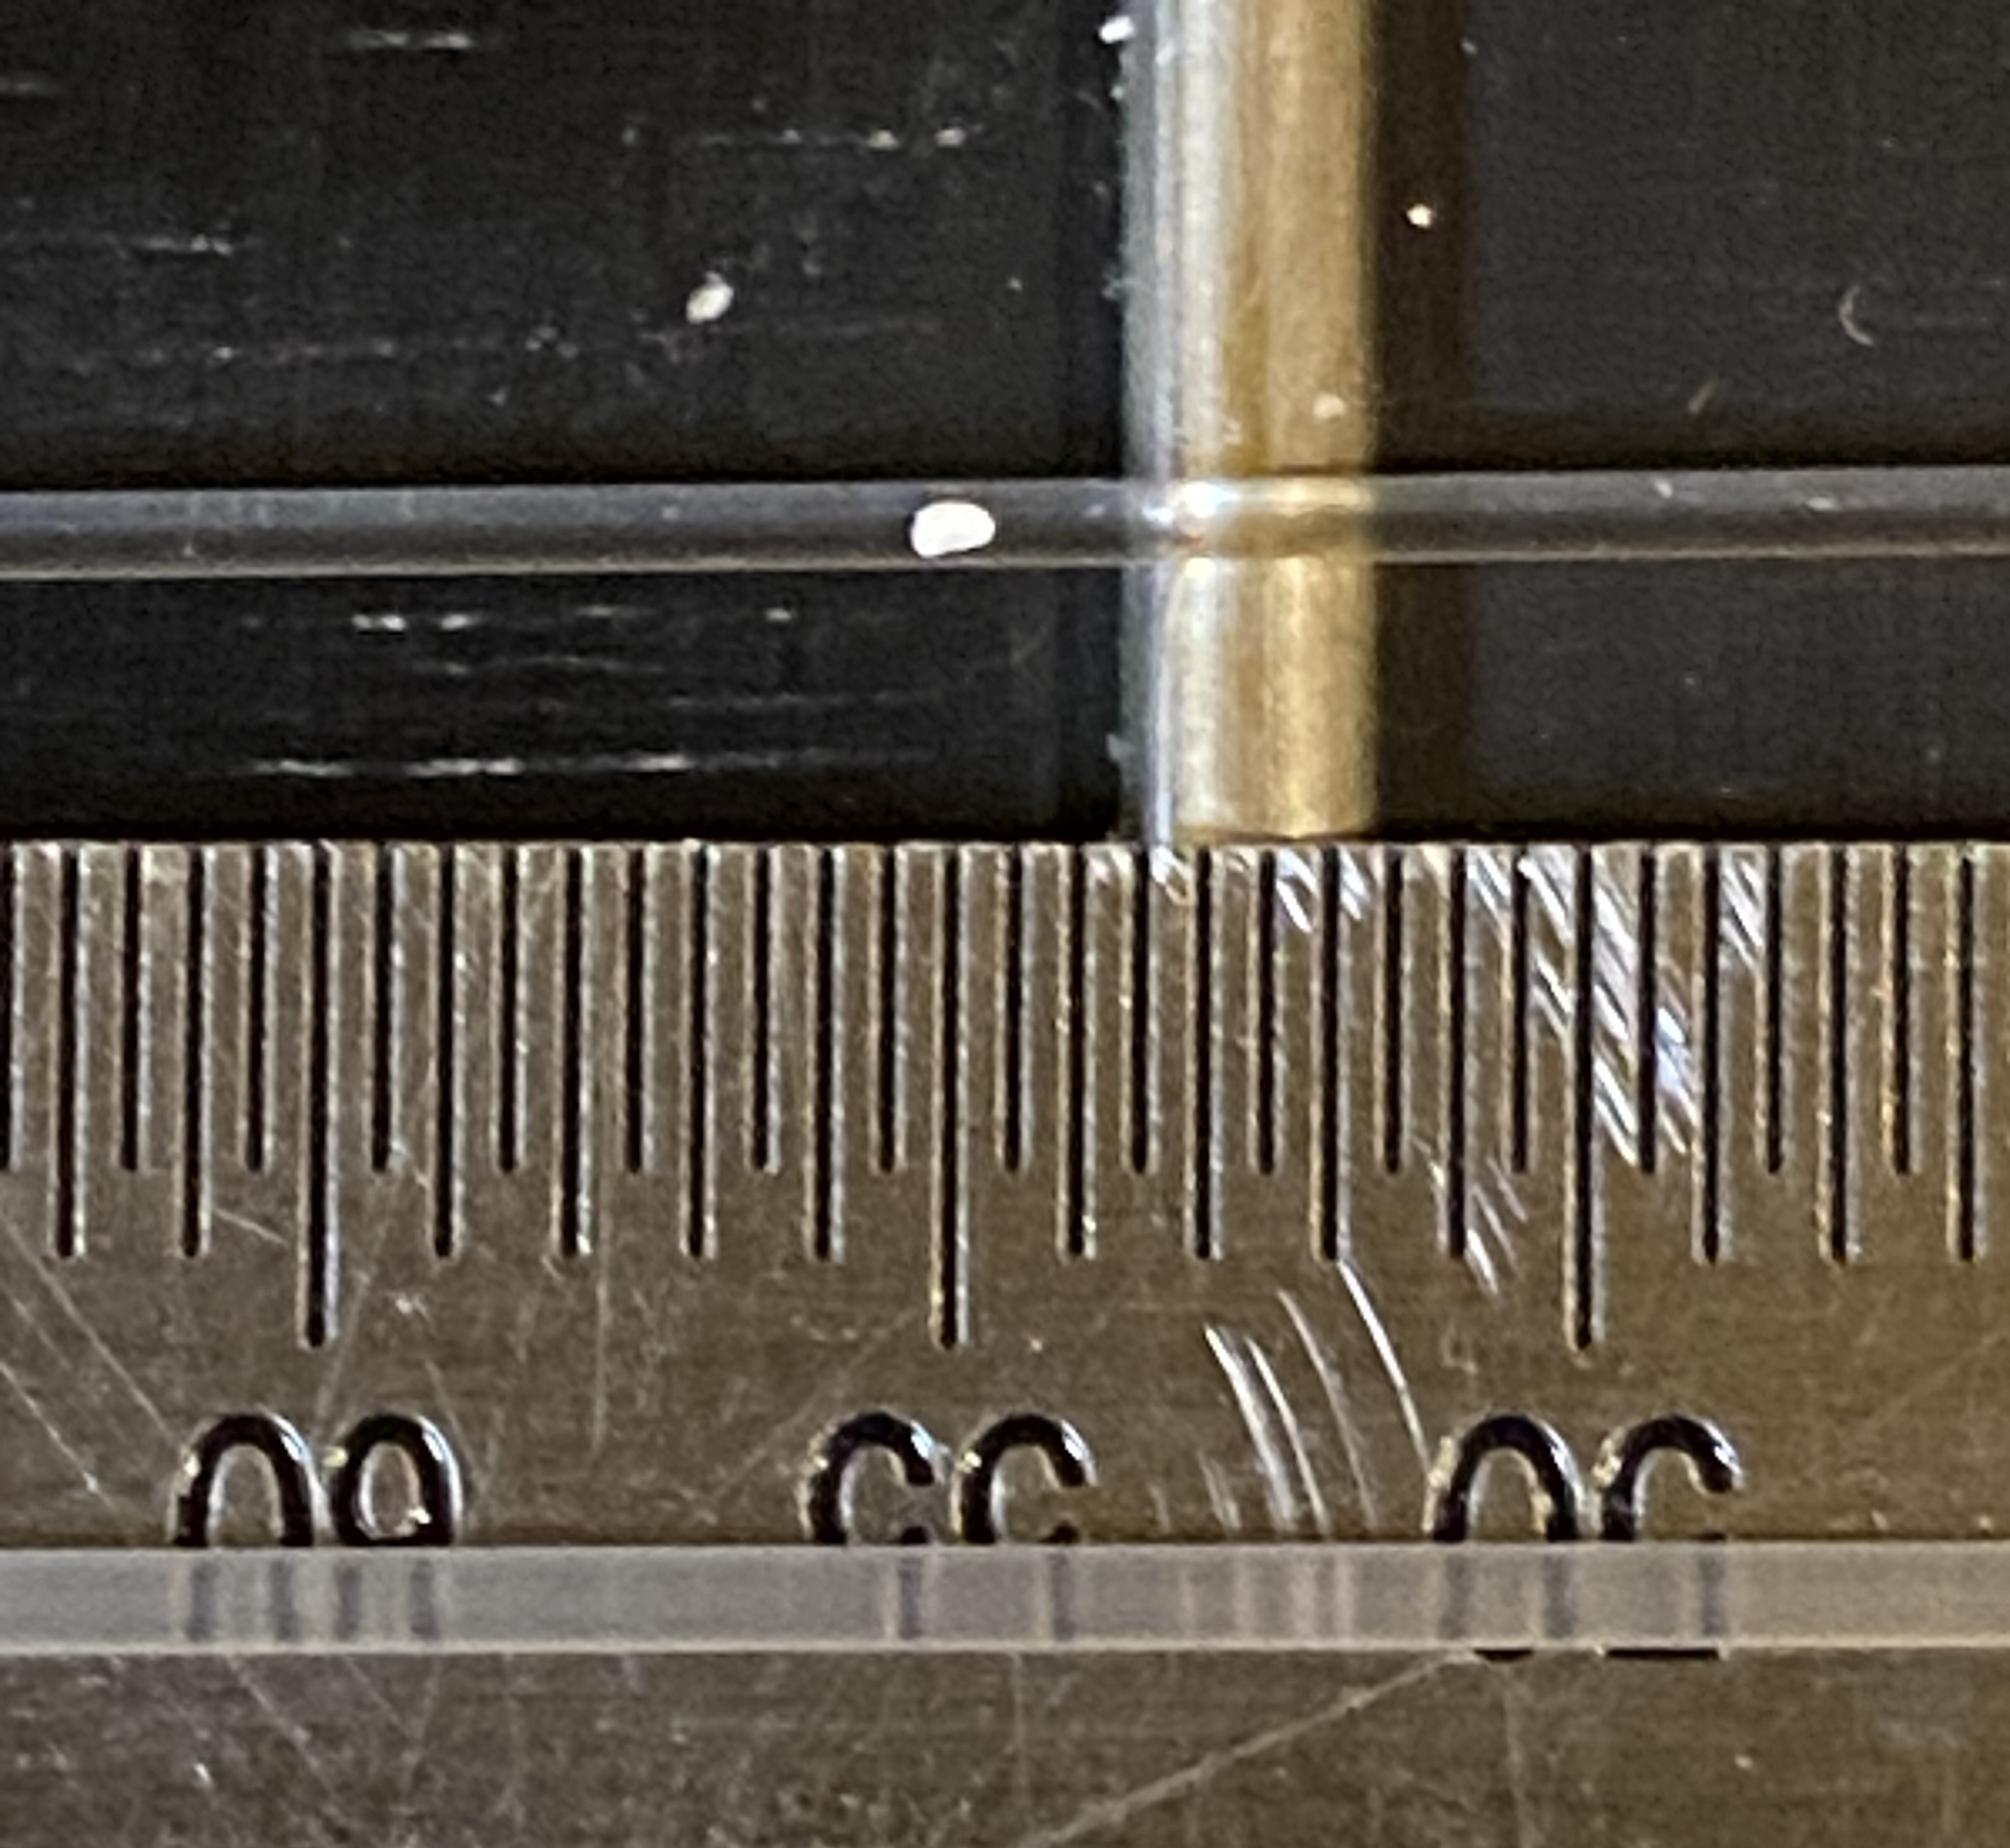
\includegraphics[width=3.04in]{figures/exp_dx2.jpg}
      \caption{$\Delta x_2$}
      \label{fig:exp_dx2}
  \end{subfigure}
  \caption{\label{fig:exp_dx} Two examples of displacement measurements of a small deposit of white correction fluid relative to a D'Addario string-depth gauge marked in half-millimeter increments.}
\end{figure}

\begin{table}
  \centering
  \caption{\label{tbl:ej45_mks} String specifications for the D'Addario Pro-Arte Nylon Classical Guitar Strings -- Normal Tension (EJ45). The corresponding scale length is 650~mm.}
  \begin{tabular}{cccccc}
\toprule
String & Note & Radius (mm) & Density ($\times 10^{-7}$ kg/mm) & Tension (N) \\
\midrule
J4501 & E$_{4}$ & 0.356 & 3.74 & 68.6 \\
J4502 & B$_{3}$ & 0.409 & 5.05 & 52.0 \\
J4503 & G$_{3}$ & 0.512 & 8.36 & 54.3 \\
J4504 & D$_{3}$ & 0.368 & 19.21 & 70.0 \\
J4505 & A$_{2}$ & 0.445 & 32.90 & 67.3 \\
J4506 & E$_{2}$ & 0.546 & 54.72 & 62.8 \\
\bottomrule
\end{tabular}


\end{table}%

It is relatively easy to measure \emph{in situ} the value of $R$ (and therefore infer $\kappa$ and $B_0$) for any guitar string with the aid of a  device that can measure frequency~\cite{ref:pgtweb}, a simple ruler with fine markings (e.g., a string depth gauge), a magnifying glass or camera with a macro mode, and white correction fluid. For example, in \fig{exp_dx} we show photographs of the nylon normal-tension first string on an Alhambra 8P classical guitar. By depositing a small sample of correction fluid on the string, we can measure small displacements against a gauge marked in half-millimeter increments. Then we can pluck the open string and measure its vibration frequency. All of our measurements were made with strings that had settled into equilibrium after at least ten hours of use, and we completed each set of measurements of a string in less than 10 minutes so that it did not have time to relax further~\cite{ref:blanc1996nvb,ref:lynchaird2017mpn}. We found that significantly stretching a string that had settled into equilibrium resulted in a nonlinear frequency shift $\Delta f$ as a function of $\Delta L$ (and occasionally broke the string). Therefore, prior to our measurements we tuned each string down one whole step by turning the tuning machine down five half-turns, stretching the string vertically to pull it through the nut, and then re-tensioning the string with two half-turns. The string stretches uniformly along its length, so at any position $x$ the relative displacement $\Delta x/x$ should be invariant. For convenience, we therefore chose to work near the first fret as a visual marker, which is located 614~mm from the saddle on a guitar with a 650~mm scale length. We made seven measurements of displacement over a 3~mm range (100 times the stretch that results from normal fretting), as well as the corresponding frequencies.

\begin{figure}
  \centering
  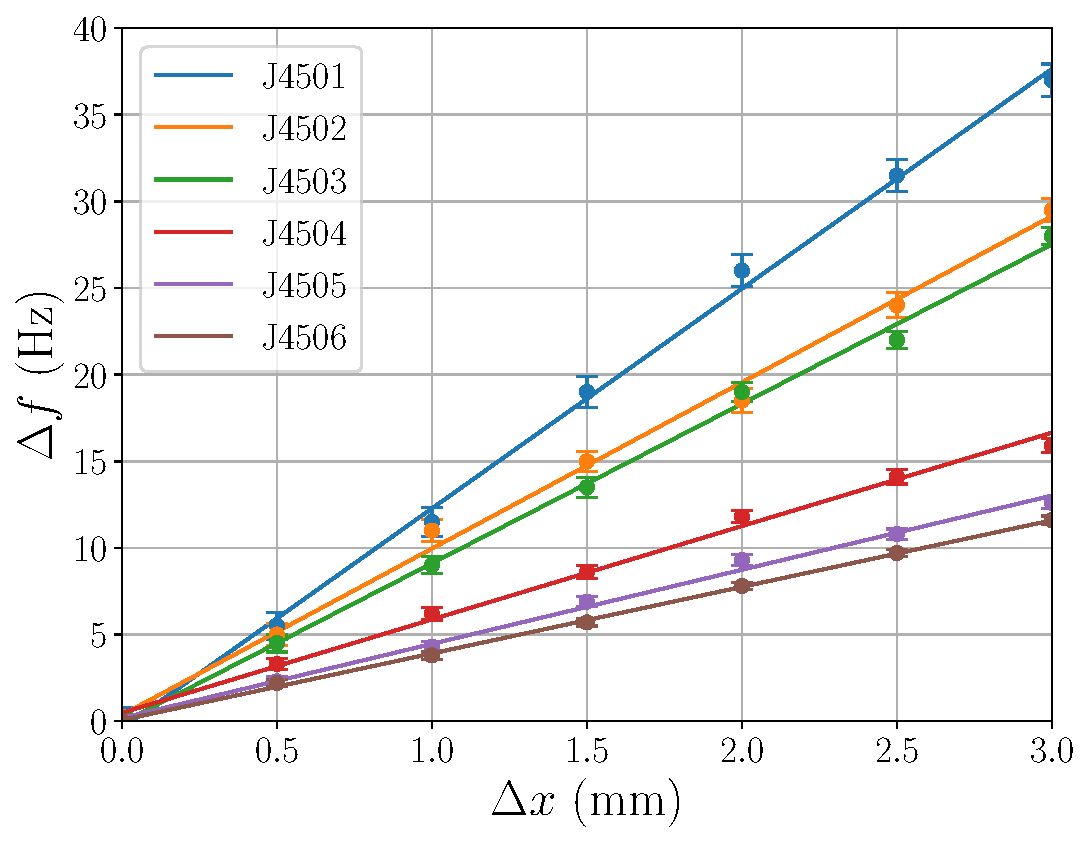
\includegraphics[width=5.0in]{figures/fit_ej45}
  \caption{\label{fig:fit_ej45} Results of experiments to measure $R$ for each string in the D'Addario Pro-Arte Nylon Classical Guitar Strings -- Normal Tension (EJ45) set. The points represent the measurement data, while the lines are the results of linear least-squares fits to that data.}
 \end{figure}

For example, we began with a normal-tension nylon classical string set~\cite{ref:daddariostcweb} with the specifications listed in \tbl{ej45_mks} using metric units.\footnote{Note that the correct unit of force in the metric system is Newtons (N), rather than kilograms, which is a unit of mass. In the British Imperial measurement system, the common units of mass are known as the ``slug'' and the ``blob.''} In \fig{fit_ej45}, we plot our measurements of $\Delta f$ as a function of the displacement $\Delta x$ relative to the frequency of the string when $\Delta x = 0$. We have not included error bars, because they are all identical: we found that 10 measurements are sufficient to reduce statistical errors in frequency (which arise primarily because of imperfect measurements of $\Delta x$) to about 0.5~Hz. We then performed a least-squares fit to a straight line~\cite{ref:bevington2003dre} (also shown in \fig{fit_ej45}), determined the derivative $\Delta f / \Delta L$, and then computed $R$ using \eqn{r_def} with $L = 614$~mm and $f$ defined as the average frequency over the range. The results are shown in \tbl{ej45_props}. Here $\sigma$ is the covariant (diagonal) uncertainty in $R$ (so that, for example, the first string in the table has $R = 23.6 \pm 0.5$), and $\kappa = 2 R + 1$. We also estimate an effective (differential) modulus of elasticity $E_\mathrm{eff}$ from \eqn{kappa_def}, expressed in units of gigapascals (1 GPa = $10^9$~N/m$^2$.). Similar measurements and results for other string sets are provided in \app{specs}. Note --- as predicted in \sct{tot_freq_shift} and shown in \fig{hist_r} for all strings sets \emph{except} the light tension set --- the expectation that the guitar will be \emph{tunable} results in $R$ values of manufactured strings that are in the range $20 - 30$. (It is unclear why the light strings appear to have much higher $R$ values. Their volume densities are within a few percent of those of the normal tension strings, so perhaps there's a significant difference in the manufacturing process.) The still more important requirement that the guitar be \emph{playable} leads us to the discussion of compensation in the next section.

% First, we tune the open string to the correct 12-TET frequency. Then, we select a fret $n$, and measure the frequency deviation $\Delta \nu_n$ of the fretted string while muting the other strings to eliminate sympathetic vibrations. If we solve \eqn{b_0_kappa} for $\kappa$ and then substitute the result into \eqn{error_tot}, we find
% \begin{equation} \label{eqn:root_kappa_quad}
%   \alpha\, B_0^2 + \beta\, B_0 - \xi = 0\, ,
% %  \alpha\, \kappa + \beta\, \sqrt{\kappa} - \xi = 0\, ,
% \end{equation}
% where we have included the quadratic bending stiffness term, and defined the coefficients
% \begin{subequations}
%   \begin{align}
%     % \alpha &\equiv \half \left[ Q_n + \left(\gamma_n^2 - 1\right)\left(1 + \pi^2\right)\left(\frac{\rho}{2\, L_0}\right)^2 \right]\, , \\
%     % \beta &\equiv \left(\gamma_n - 1\right)\, \frac{\rho}{2\, L_0}\, , \nd \\
%     % \xi &\equiv \frac{\ln(2)}{1200}\, \Delta \nu_n + \frac{\left(\gamma_n - 1\right) \Delta S - \Delta N}{X_0}\, .
%     \alpha &\equiv \half \left[ \left(\frac{2\, L_0}{\rho}\right)^2 Q_n + \left(\gamma_n^2 - 1\right)\left(1 + \pi^2\right) \right]\, , \\
%     \beta &\equiv \gamma_n - 1\, , \nd \\
%     \xi &\equiv \frac{\ln(2)}{1200}\, \Delta \nu_n + \frac{\left(\gamma_n - 1\right) \Delta S - \Delta N}{X_0}\, .
% \end{align}
% \end{subequations}
% \Eqn{root_kappa_quad} is quadratic in $B_0$, with the solution
%  \begin{equation} \label{eqn:root_kappa_soln}
% B_0 = \frac{\sqrt{\beta^2 + 4\, \alpha\, \xi} - \beta}{2\, \alpha} \approx \frac{\xi}{\beta}\, ,
%  \end{equation}
% where we have chosen the positive root to ensure that $B_0 > 0$, and the final approximate expression on the \rhs applies when $\beta^2 \gg 4\, \alpha\, \xi$.

% We've used this approach to estimate $\kappa$ and $R$ of different string sets on the Alhambra 8P classical guitar, which has $X_0 = 650$~mm, $c = 3.5$~mm, $\Delta S = 1.5$~mm, and $\Delta N = 0.0$~mm. At the nut, $b = 1.0$~mm, but the height of the fret board decreases roughly linearly further toward the saddle, effectively increasing $b$. We estimate that $d b / d x \approx -0.0034$, so that $b$ has increased to 2.0~mm at the 12$^{\text{th}}$ fret. . In \tbl{ej45_props}, we list the frequency deviation from 12-TET at the 12$^{\text{th}}$ fret for each string in this set, as well as the corresponding estimates of $\kappa$, $R$, $E$, and $B_0$, computed from \eqn{root_kappa_soln}, \eqn{r_def}, \eqn{kappa_def}, and \eqn{b_0_kappa}, respectively.

\begin{table}%[htbp]
  \centering
  \caption{\label{tbl:ej45_props} Derived physical properties of the D'Addario Pro-Arte Nylon Classical Guitar Strings -- Normal Tension (EJ45). The corresponding scale length is 650 mm.}
  \begin{tabular}{cccccc}
\toprule
String & $R$ & $\sigma$ & $\kappa$ & $B_0$ & $E$ (GPa) \\
\midrule
J4501 & 23.6 & 0.5 & 48.2 & 0.00190 & 8.33 \\
J4502 & 23.8 & 0.7 & 48.6 & 0.00219 & 4.81 \\
J4503 & 28.8 & 0.7 & 58.7 & 0.00302 & 3.87 \\
J4504 & 22.4 & 0.8 & 45.7 & 0.00192 & 7.51 \\
J4505 & 23.8 & 0.8 & 48.6 & 0.00238 & 5.27 \\
J4506 & 28.6 & 0.4 & 58.2 & 0.00321 & 3.90 \\
\bottomrule
\end{tabular}


\end{table}%

\begin{figure}
  \centering
  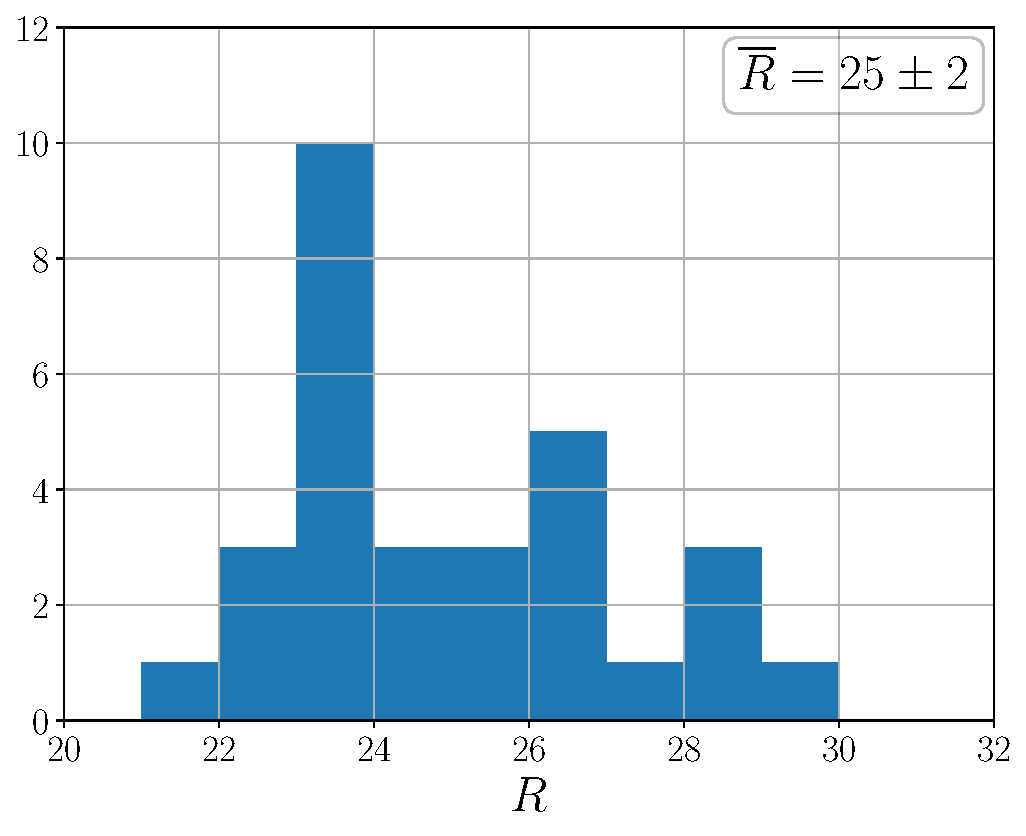
\includegraphics[width=5.0in]{figures/hist_r}
  \caption{\label{fig:hist_r} A histogram of the parameter $R$ for all strings \emph{except} those in the nylon light tension set presented in \app{specs_ltn}, which seem to have anomalously high values.}
\end{figure}

\begin{figure}
  \centering
  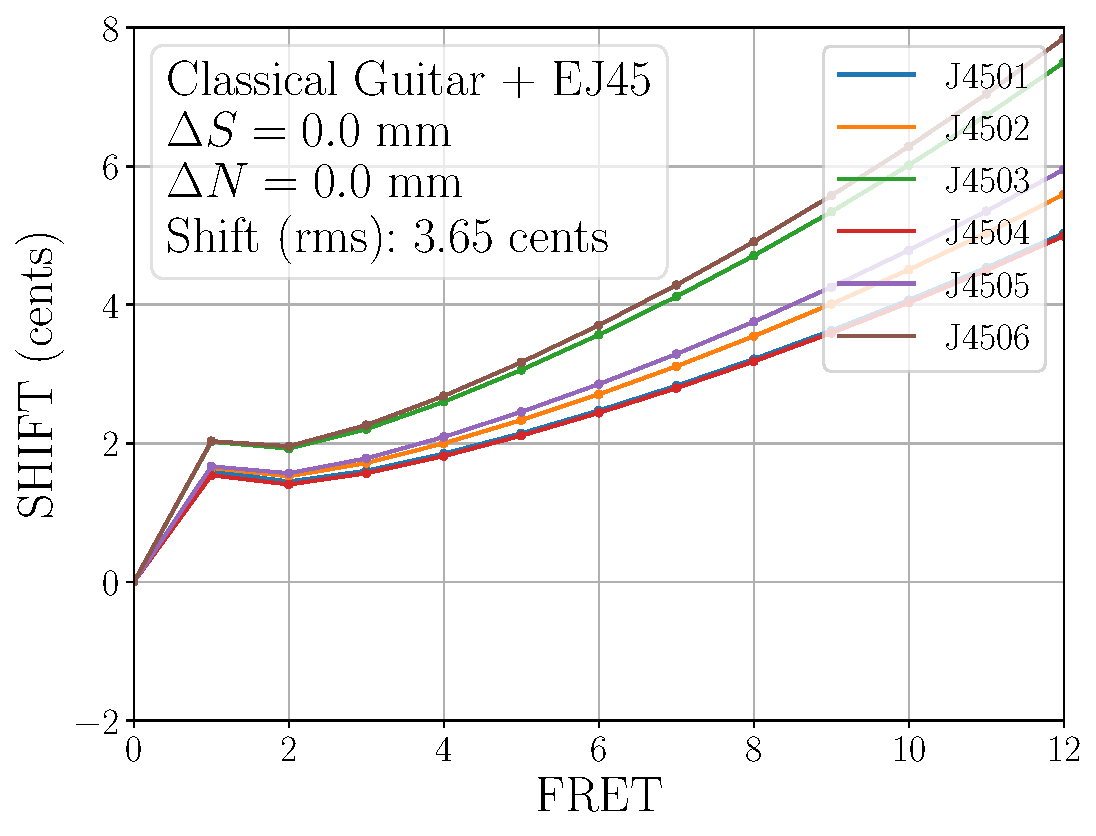
\includegraphics[width=5.0in]{figures/shift_classicalguitar_ej45_null}
  \caption{\label{fig:shift_classicalguitar_ej45_null} Frequency errors for an uncompensated Classical Guitar with normal tension nylon strings (D'Addario EJ45).}
\end{figure}

Adopting these physical properties of the normal string set and applying them to a computation of the frequency deviations for our standard classical guitar, we obtain the predictions shown in \fig{shift_classicalguitar_ej45_null} using \eqn{error_def}. Anticipating our treatment of exact compensation in \sct{comp} and \app{rms}, we compute the root-mean-squared (RMS) average of the frequency deviations for each string. This mean (over the first 12 frets) can be computed by squaring the frequency deviations shown in \fig{shift_classicalguitar_ej45_null}, averaging those values, and then taking the square root of the result.

Recall that we recalculated the expected frequency shift of a classical guitar string with asymmetric boundary conditions in \app{freq}, and found an expression for $f_q$ given by \eqn{f_m_hybrid} that reduces --- by about a factor of 2 --- the impact of the bending stiffness relative to the symmetric (clamped) case in \eqn{f_m_clamped}. Furthermore, we have not used more sophisticated techniques to calculate the bending stiffness for either monofilament nylon strings or wound nylon strings, opting instead for the phenomenological model given by \eqn{b_0_kappa}. But is this approach valid? As a test, we compared our frequency shift estimates based on \sct{model} with experimental measurements made using five different guitars 

result in very large frequency deviations at all frets. As shown in \fig{japan_guitar_ej45_shifts}, we measured the shifts at the first fret and found that they fell into the range of $4.5 - 5.75$~cents, consistent with our predictions. At the 12$^\mathrm{th}$ fret, we measured $\Delta f = 18.5 - 19.5$~cents for the third and sixth strings, and $\Delta f = 15.75 - 17.5$~cents for the other strings, in reasonably close agreement with our predictions. By contrast, the corresponding equation arising from symmetric (clamped) boundary conditions --- \eqn{f_m_clamped} --- predicts shifts that are $30 - 45$\% higher, and setbacks that are more than a factor of two larger. We conclude that \eqn{f_m_hybrid} and \eqn{b_0_kappa} can be used to reliably predict setbacks for classical guitars.

%Recall how we introduced this concept in \sct{model_tension}: increasing the tension by a quantity $\Delta T$ causes a shift in the frequency of a guitar string by $\Delta \nu$ in cents. Although we were considering fretted strings when we derived \eqn{error_def}, the terms in that equation can be generalized to describe the case of an open string that has been stretched longitudinally. Suppose that we continue to clamp the string at the saddle and the nut, but that we tighten the tuning gear to stretch that string's length by an amount $\Delta L$. The change in the string's frequency due to the change in the open resonant length is zero, because $L_0 / \gamma_0 L_0 = 1$. The linear mass density of the string is smaller now because there is less material between the saddle and the nut, causing the frequency shift (in cents)
% \begin{equation}
%600\, \log_2 \left(  \frac{\mu}{\mu + \Delta \mu} \right) \approx \frac{600}{\ln(2)}\, \frac{\Delta L}{L}\, ,
% \end{equation}
%where $L$ is the initial length of the string. Finally, the tension in the string increases by $\Delta T$ due to the elastic properties of the string. Following the discussion in \sct{model_tension}, the corresponding frequency shift  is
% \begin{equation}
%600\, \log_2 \left(  \frac{T + \Delta T}{T} \right) \approx \frac{600}{\ln(2)}\, \frac{\Delta L}{L}\, \kappa\, ,
% \end{equation}
%where $T$ is the initial tension of the string. Therefore, the total frequency shift of the open string caused by a change $\Delta L$ in the string's length is
% \begin{equation}
%\Delta \nu \approx \frac{600}{\ln(2)}\, \frac{\Delta L}{L}\, (\kappa + 1)\, ,
% \end{equation}
%characterizing the string frequency's response to a change in length. It is dominated by the change in the tension of the string, and given $R$ we can quickly determine $\kappa$.
%
%
%Solving this expression for the string constant, we find
% \begin{equation}
%\kappa = \frac{\ln(2)}{600}\, R - 1\, ,
% \end{equation}
%where
% \begin{equation}
%R \equiv \frac{L}{\Delta L}\, \Delta \nu
% \end{equation}
%is a parameter originally defined by Byers\footnote{Byers expressed this parameter in terms of the fractional frequency shift (in Hertz) as $R = (L/\Delta L) (\Delta f/f) \approx (\ln(2)/1200) (L/\Delta L) \Delta \nu$. Therefore, our dimensionless value of $R$ is larger than Byers' by a factor of about 1730.}~\cite{ref:byers1996cgi,ref:varieschi2010icf}.

% \begin{equation}
% \begin{split}
%L_{n \ge 1}(y) &= \sqrt{\left(X_n + \Delta S\right)^2 + (b + c)^2 + y^2} \\
%&\approx X_n + \Delta S + \frac{(b + c)^2 + y^2}{2\, X_n}\, .
% \end{split}
% \end{equation}
%
% \begin{equation}
% \begin{split}
%L^\prime_{n \ge 1}(y) &= \sqrt{\left(X_0 - X_n + \Delta N\right)^2 + b^2 + y^2} \\
%&\approx X_0 - X_n + \Delta N + \frac{b^2 + y^2}{2 \left(X_0 - X_n\right)}\, .
% \end{split}
% \end{equation}
%
% \begin{equation}
% \begin{split}
%Q_n(y) &\approx \frac{1}{2\, X_0} \left[ \frac{(b + c)^2 + y^2}{X_n} + \frac{b^2 + y^2}{X_0 - X_n} - \frac{c^2}{X_0} \right] \\
%&= Q_n(0) + \Delta Q_n(y) \, ,
% \end{split}
% \end{equation}
%where $Q_n(0)$ is given by \eqn{lambda_n_approx}, and
% \begin{equation}
%\Delta Q_n(y) \equiv \frac{1}{2 \left(\gamma_n - 1\right)}\, \left(\frac{\gamma_n\, y}{X_0}\right)^2\, .
% \end{equation}
%
%Following the same approach we used to derive \eqn{quad_shift}, we can derive the change in the total shift due to both resonant length and linear mass density for a transverse displacement $y$. To second order in $y$, we find that
% \begin{equation}
%\Delta \nu_n(y) \approx \frac{600}{\ln(2)}\, \frac{3 - 2 \gamma_n}{2 \left(\gamma_n - 1\right)}\, \left(\frac{\gamma_n\, y}{X_0}\right)^2\, .
% \end{equation}
%We have plotted this expression for the first 12 frets and $y = 5$~mm in \fig{quad_shift_factory}. This shift is quite small compared to the experimental errors we'll obtain in the shifts due to tension, and we ignore it in what follows.
%
% \begin{figure}
%  \centering
%  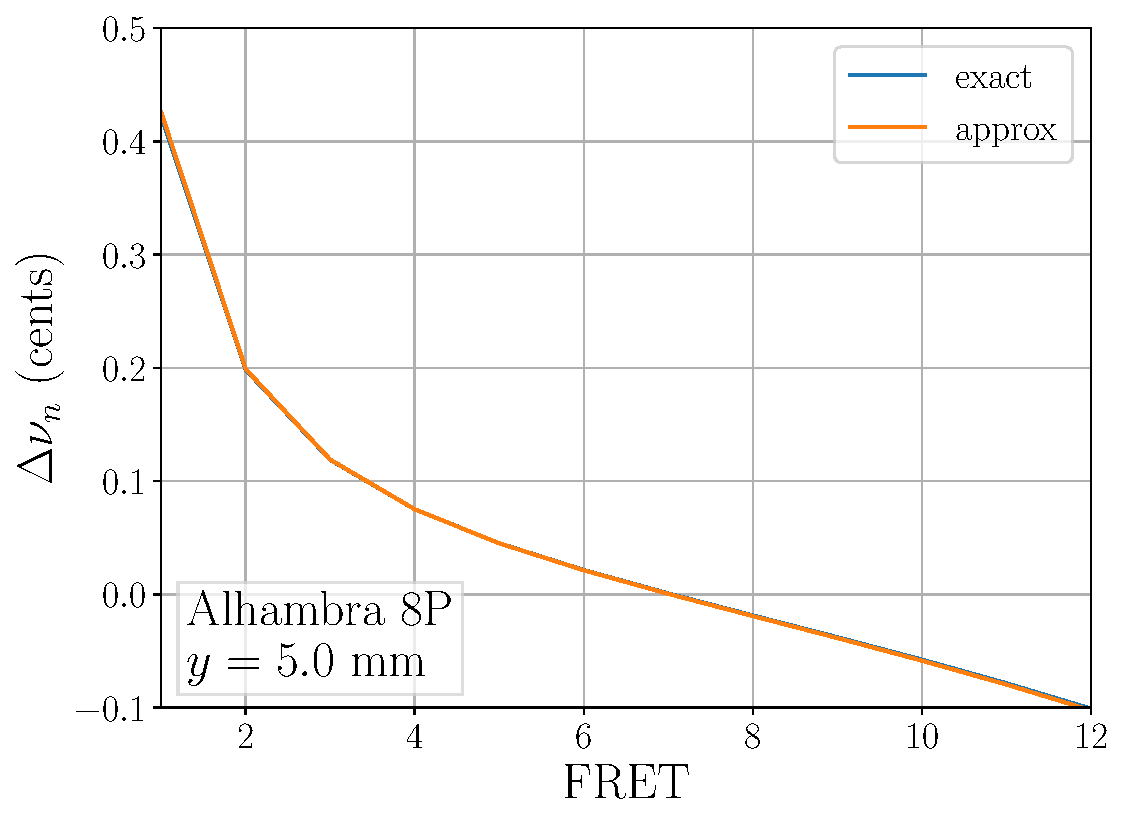
\includegraphics[width=5.0in]{figures/quad_shift_factory}
%  \caption{\label{fig:quad_shift_factory} Total frequency shift (in cents) due to resonant length and linear mass density for a transverse displacement of $y = 5$~mm. This shift is identical for each string, and should be smaller than the experimental errors we'll accumulate using our transverse displacement approach.}
% \end{figure}
%
%\begin{table}%[htbp]
%  \centering
%  \caption{\label{tbl:ej43_props} Derived physical properties of the D'Addario Pro-Arte Nylon Classical Guitar Strings -- Light Tension (EJ43). The corresponding scale length is 650 mm.}
%    \begin{tabular}{lcccc}
%    \hline \hline
%    String  & $R$ & $\kappa$ & Modulus (GPa) & Stiffness \\
%    \hline
%    J4301 & 4.39 $\times 10^{4}$ & 49.8 & 8.62 & 3.79 $\times 10^{-3}$ \\
%    J4302 & 5.02 $\times 10^{4}$ & 57.0 & 5.62 & 4.68 $\times 10^{-3}$ \\
%    J4303 & 4.79 $\times 10^{4}$ & 54.4 & 3.57 & 5.72 $\times 10^{-3}$ \\
%    J4304 & 5.02 $\times 10^{4}$ & 57.0 & 9.52 & 4.13 $\times 10^{-3}$ \\
%    J4305 & 4.39 $\times 10^{4}$ & 49.8 & 5.05 & 4.55 $\times 10^{-3}$ \\
%    J4306 & 5.27 $\times 10^{4}$ & 59.9 & 3.97 & 6.35 $\times 10^{-3}$ \\
%    \hline
%    \end{tabular}%
%  \label{tab:addlabel}%
%\end{table}%

%\begin{table}[htbp]
%  \centering
%  \caption{\label{tbl:ej45_ips} String specifications for the D'Addario Pro-Arte Nylon Classical Guitar Strings -- Normal Tension (EJ45). The corresponding scale length is 25.5~inches.}
%    \begin{tabular}{lcccc}
%    \toprule
%    String  & Note  & \multicolumn{1}{l}{Diameter (in)} & \multicolumn{1}{l}{Density (lb/in)} & \multicolumn{1}{l}{Tension (lb)} \\
%    \midrule
%    J4501 & $E_4$  & 0.0280 & $2.092 \times 10^{-5}$ & 15.3 \\
%    J4502 & $B_3$  & 0.0322 & $2.827 \times 10^{-5}$ & 11.6 \\
%    J4503 & $G_3$  & 0.0403 & $4.679 \times 10^{-5}$ & 12.1 \\
%    J4504 & $D_3$  & 0.0290 & $1.075 \times 10^{-4}$ & 15.6 \\
%    J4505 & $A_2$  & 0.0350 & $1.842 \times 10^{-4}$ & 15.0 \\
%    J4506 & $E_2$  & 0.0430 & $3.063 \times 10^{-4}$ & 14.0 \\
%    \bottomrule
%    \end{tabular}%
%\end{table}%
